\chapter{Wybrany model ciała miękkiego}

\section{Kryteria wyboru modelu}

Wybór metody symulacji uzależniony jest od zakresu zjawisk fizycznych które mają
być jej przedmiotem. Zanim przedstawiona zostanie wybrana metoda symulacji
wymienione będą kryteria którymi kierowałem się przy wyborze.
Pragnę też zaznaczyć, że wybór nastąpił w głównej mierze metodami empirycznymi,
większość z poznanym metod została zaimplementowana i w przypadku niemożności
uzyskania porządanych efektów wizualnych lub wydajnościowych wyszukiwana była
inna.

Pierwszym kryterium jakim kierowałem się przy wyborze metody było
zawężenia przedmiotu symulacji do ciał posiadających objętość. Wiele z
metod ukierunkowanych na symulację włosów czy materiałów musiały zostać odrzucone ze
względu na posiadane przez nie własności niestosowalne w
symulacji obiektów z objętości - np. podatność na marszczenie. Nie oznacza to
natomiast, że nie istnieją metody mogące symulować oba zjawiska - przykładem
jest chociażby System Sprężyn omawiany w rozdziale 2.

Kolejnym kryterium, a właściwie uproszczeniem było założenie, że
symulowany obiekt będzie jednorodny pod względem wypełnienia, czy inaczej,
materiału z którego jest zbudowany. Pozwala to na
uniknięcia modelowania, często nietrywialnego, właściwości fizycznych modelu, co z pewności
wykroczyłoby poza temat tej pracy. 

% złożone obiekty o skomplikowanej siatce
Innym istotnym wymaganiem jest umożliwienie symulowania obiektów
przygotowanych w programach do modelowania 3D. Obiekty takie często składają się
wielu tysięcy wierzchołków, które posiadają własne współrzędne teksturowania,
czy normalne. Implikacją tego założenia jest fakt, że poszukiwana metoda musi być
metodą Lagrange'a symulującą dynamikę wierzchołków trójwymiarowego modelu.
Dodatkowe informacje związane z modelem, takie jak połączenia między
wierzchołkami czy wierzchołki tworzące trójkąty mogły być wykorzystane w
symulacji.

% zakres degeneracji
Każde symulowane ciało miękkie poddane działaniu sił może zostać odkształcone
tylko w zdefiniowanym zakresie. W przypadku gdy siły zewnętrzne przestają działać
na ciało, siły wewnętrzne powinny sprowadzić obiekt do formy nieodkształconej.
Takie założenie upraszcza symulację gdyż wyklucza trwałą degenerację siatki
obiektu.

% przeznaczona do symulacji czasu rzeczywistego stabilna do zastosowań
Najważniejszym wymaganiem jakie brane było pod przy wyborze metody jest możliwość
zastosowania do symulacji czasu rzeczywistego. Metody złożone obliczeniowo takie
jak przytaczane w rozdziale 2 Metody Continuum nie spełniają tego kryterium.
Również metody wymagające zaawansowanej obróbki modelu - takie jak np. System
Sprężyn wymagają zdefiniowania wewnętrznej struktury obiektu, co wiąże się z
generowaniem znacznej ilości cząstek poddanych symulacji. 

Z moich eksperymentów z wypełnianiem modelu sześcienną siatką i użyciem Systemu Sprężyn wynika, że
gęste wypełnienie średniej złożoności modelu punktami wewnętrznymi powoduje
zbytnie usztywnienie obiektu i znacząco spowalnia symulację. W przeciwieństwie,
gdy wnętrze modelu jest rzadko wypełnione cząstkami wewnętrznymi wyjściowa
siatka modelu podlega znacznej degeneracji. Znalezienie optymalnej gęstości
siatki odbywało się drogą eksperymentów.

% skalowana do gpu
Tematem tej pracy jest poznanie i zastosowanie technologii CUDA. Dlatego też
ostatnim kryterium jakie brane było pod uwagę przy wyborze metody symulacji jest
możliwość wykorzystania GPU do obliczeń. Wymaga to aby
przetwarzanie danych w wybranej metodzie odbywało się możliwie lokalnie, co
pozwoli na zrównoleglenie obliczeń i uzyskanie wzrostu wydajności.

% skad wzialem metode czyja to, kiedy skad
Jako źródło informacji o dostępnych metodach wykorzystywany był głównie
internet. Jak to zostało wcześniej napisane, nie są znane mi żadne książki
poruszające tematykę symulacji ciał miękkich w grafice komputerowej. Mimo
niedostępności poszukiwanego kompendium wiedzy dostępne są trzy bardzo dobre
artykuły stanowiące przekrój przez szereg opublikowanych metod: \cite{TR97-19},
	\cite{pbdo}, \cite{survey}. Cennym źródłem informacji są też materiały
	publikowane konferencyjne publikowane na stronie \textit{www.siggraph.org}.

% klasyfikacja tej metody - Lagrange geometryczno fizyczny
Zaimplementowana w tej pracy metoda bazuje głównie na artykule \textit{Robust
	Real-Time Deformation of Incompressible Surface Meshes}\cite{diziol},
opublikowanym na konferencji SIGGRAPH w 2011r. Wybrana metoda jest wg
klasyfikacji z rozdziału 2 metodą Lagrange'a posiadająca zarówno elementy
fizyczne jak i niefizyczne. Elementami fizycznymi jest pojawianie się sił w
momencie gdy obiekt zmienia swoją objętość oraz siły grawitacji. Za część
niefizyczną, uznany jest tzw. \textit{Shape Matching}, czyli metoda geometryczna
oddziałująca na cząstki modelu w taki sposób aby zminimalizować ich odchylenie
ich położeń od stanu wejściowego.

% dlaczego powinna byc szybka nie potrzeba wypelniac obiektu puntkami - operuje bezposrednio na powierzchni siatki
Ważniejszą jednak zaletą wybranego modelu jest fakt, że w przeciwieństwie do
Systemu Sprężyn symulowane obiekty nie muszę mieć
zdefiniowanej struktury wewnętrznej. Pozwala to znacząco przyspieszyć symulację
unikając generowania znacznej ilość cząstek, które odpowiadają tylko za
utrzymanie fizycznych właściwości obiektu. Metoda ta operuje bezpośrednio na
trójkątnej siatce, co pozawala wczytać obiekt bezpośrednio z formatu modeli
3D.

% dlaczego powinna byc stabilna - brak sil, dynamika z constraintami
Kolejną zaletą użytej techniki symulacji jest jej stabilność. Wynika ona z
operowania metody bezpośrednio na pozycjach cząstek zamiast na siłach. Pozwala
to na bardzo prostą implementację reakcji na zderzenia z innymi obiektami czy
samym sobą. Dokładniejszy opis schematu symulacji układu w czasie będzie w
dalszej części tego rozdziału.

% dlaczego jest dobra na gpu
Ostatnią zaletą jest też możliwość efektywnej implementacji wybranej metody na
procesorach graficznych. Dobra lokalność przetwarzanych danych sprawia, że
możliwe jest pełne wykorzystanie procesora graficznego, co w połączeniu z
techniką redukcji złożoności algorytmu zaproponowaną przez autorów, czyni ją
idealną do zastosowania w symulacjach czasu rzeczywistego.

\section{Zachowanie kształtu}
Dopasowanie kształtu (ang. Shape Matching) jest geometryczną techniką
zaproponowaną po raz pierwszy w 2005 r. przez Muller'a \cite{shape}. Służy ona do
symulowania sił wewnętrznych ciała poddanemu deformacji. Metoda ta zamiast
generować siły działające na cząstki, tak jak to ma miejsce w przypadku
sprężyn w modelu Systemu Sprężyn, definiuje docelowe pozycje cząstek - $g_i$.
Pozycje te powstają w wyniku próby dopasowania konfiguracji 
pozycji cząstek ciała w stanie niezdeformowanym do aktualnej.

Wyliczone docelowe pozycje $g_i$ wykorzystywane są w symulacji do "przyciągania"
aktualnych pozycji cząstek. W przypadku gdy docelowe pozycje cząstek stają się
natychmiastowo aktualnymi uzyskamy efekt dynamiki ciała sztywnego.

\begin{figure}[ht]
\centering
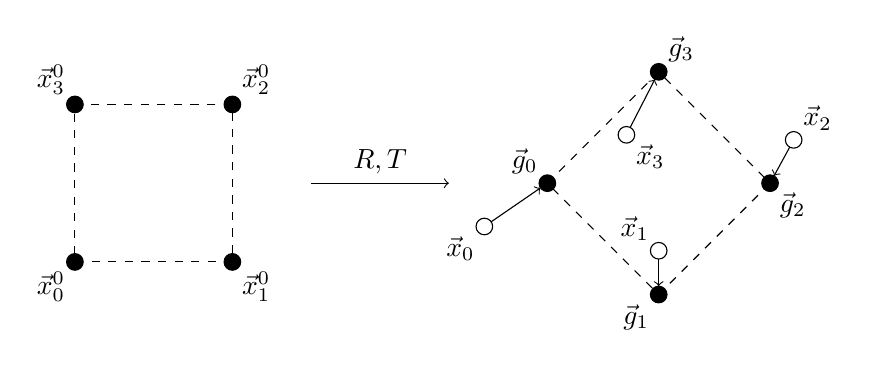
\begin{tikzpicture}

	\coordinate (A) at (0, 0, 0);
	\coordinate (B) at (2, 0, 0);
	\coordinate (C) at (2, 2, 0);
	\coordinate (D) at (0, 2, 0);

	\draw[-,dashed] (A) -- (B) -- (C) -- (D) -- (A);

	\filldraw[fill=black, draw=black] (A) circle (3pt);
	\filldraw[fill=black, draw=black] (B) circle (3pt);
	\filldraw[fill=black, draw=black] (C) circle (3pt);
	\filldraw[fill=black, draw=black] (D) circle (3pt);

	\node[above left] at (D) {$\vec{x}^0_3$};
	\node[below right] at (B) {$\vec{x}^0_1$};
	\node[above right] at (C) {$\vec{x}^0_2$};
	\node[below left] at (A) {$\vec{x}^0_0$};

	% arrow
	\coordinate (R1) at (3, 1, 0);
	\coordinate (R2) at (4.75, 1, 0);
    \draw[->] (R1) -- (R2) node[midway,above] {$R, T$};

	% transformed

	\coordinate (A1) at (6, 1, 0);
	\coordinate (B1) at (7.4142, 2.4142, 0);
	\coordinate (C1) at (8.8284, 1, 0);
	\coordinate (D1) at (7.4142, -0.4142, 0);

	\draw[-,dashed] (A1) -- (B1) -- (C1) -- (D1) -- (A1);

	\filldraw[fill=black, draw=black] (A1) circle (3pt);
	\filldraw[fill=black, draw=black] (B1) circle (3pt);
	\filldraw[fill=black, draw=black] (C1) circle (3pt);
	\filldraw[fill=black, draw=black] (D1) circle (3pt);

	\node[below left] at (D1) {$\vec{g}_1$};
	\node[above right] at (B1) {$\vec{g}_3$};
	\node[below right] at (C1) {$\vec{g}_2$};
	\node[above left] at (A1) {$\vec{g}_0$};

	\coordinate (X1) at (5.2, 0.45, 0);
	\coordinate (X2) at (7.0042, 1.6142, 0);
	\coordinate (X3) at (9.1284, 1.55, 0);
	\coordinate (X4) at (7.4142, 0.142, 0);

	\filldraw[fill=white, draw=black] (X1) circle (3pt);
	\filldraw[fill=white, draw=black] (X2) circle (3pt);
	\filldraw[fill=white, draw=black] (X3) circle (3pt);
	\filldraw[fill=white, draw=black] (X4) circle (3pt);

	\node[below left] at (X1) {$\vec{x}_0$};
	\node[below right] at (X2) {$\vec{x}_3$};
	\node[above right] at (X3) {$\vec{x}_2$};
	\node[above left] at (X4) {$\vec{x}_1$};

    \draw[shorten >=3pt,shorten <=3pt,->] (X1) -- (A1);
    \draw[shorten >=3pt,shorten <=3pt,->] (X2) -- (B1);
    \draw[shorten >=3pt,shorten <=3pt,->] (X3) -- (C1);
    \draw[shorten >=3pt,shorten <=3pt,->] (X4) -- (D1);

\end{tikzpicture}

\caption{Geometryczne dopasowanie kształtu do zdeformowanych punktów w Shape Matching.}
\label{shape-matching}
\end{figure}

Ideę shape matching przedstawia rysunek \ref{shape-matching}. Punkty w stanie
niezdeformowanym $x^0_i$ są dopasowywane do zdeformowanych pozycji $x_i$ za
pomocą macierzy rotacji i wektorów translacji. 
Formalnie koncepcję Shape Matchingu autorzy w \cite{shape} zdefiniowali jako problem minimalizacji
funkcji:
\begin{equation}
E^2 = \sum_{i} m_i ||R (x^0_i - t^0) - (x_i - t) ||^2,
\label{min}
\end{equation}
gdzie $t^0$ i $t_i$ są wektorami translacji, a $R$ jest macierzą
rotacji.

Przedstawiony w problem sprowadza się do minimalizacji błędu średniokwadratowego.
Wyrażenie z \ref{min} można przedstawić jako funkcję trzech zmiennych:
\begin{equation*}
\phi(R, t, t^0) = \sum_{i} m_i ||R (x^0_i - t^0) - (x_i - t) ||^2,
\end{equation*}

Okazuje się, że znalezienie wartości wektorów $t$ i $t^0$ w
wyrażeniu \ref{min} jest możliwe. Muller \cite{shape} podaje, że optymalnymi
wektorami translacji $t^0$ i $t$ są odpowiednio środek masy obiektu
niezdeformowanego (konfiguracja spoczynkowa) i środek masy
ciała w aktualnej konfiguracji. Pokazanie tego rozwiązania polega na
wyliczeniu gradientów funkcji $\phi$ po zmiennych $t$ i $t^0$ i przyrównaniu ich
do zera.

Zanim zostanie przedstawiony dowód że środki mas są optymalnymi wektorami
translacji, przypomniane zostaną wzory na pochodne cząstkowe wraz z ich
wektorowymi odpowiednikami. Zakładając że dane mamy funkcje $f: R^n \to R^m$,
$g: R^n \to R^m$ i $h = f^T g$, gdzie $h: R^n \to R^1$. Gradient
funkcji $h$ wyraża się wzorem:
\begin{equation*}
\partial h = f^T \partial g + g^T \partial f
\end{equation*}
gdzie $\partial f$ to macierz Jacobiego (pochodnych cząstkowych), a $f^T$ jest
oznaczeniem transpozycji funkcji.

W przypadku gdy funkcje $f = g$, gradient ma postać:
\begin{equation}
\partial h = 2 f^T \partial f,
\label{part}
\end{equation}

Wprowadzając nowe oznaczenia:
$$ v = R (x^0_i - t^0) - (x_i - t)$$
$$ \phi = \sum_i m_i v^T v$$ 
i uwzględniając własność \ref{part}, gradient funkcji $\phi$ po
zmiennych $t^0$ i $t$ zapiszemy:
\begin{eqnarray*}
\nabla_{t^0} \phi = 2 \sum_i m_i (R (x^0_i - t^0) + t - x_i)^T (-R)\\
\nabla_{t} \phi = 2 \sum_i m_i (R (x^0_i - t^0) + t - x_i)^T\\
\end{eqnarray*}

Transponując obie strony otrzymujemy:
\begin{eqnarray*}
\nabla_{t^0}^T \phi = -2 \sum_i m_i R^T (R (x^0_i - t^0) + t - x_i)\\
\nabla_{t}^T \phi = 2 \sum_i m_i (R (x^0_i - t^0) + t - x_i)\\
\end{eqnarray*}

W celu wyliczenia wartości $t$ i $t^0$ przyrównujemy gradient do zera:
\begin{eqnarray}
\label{d1}
\nabla \phi_{t^0} = 0 \Leftrightarrow \sum_i m_i R^T (R (x^0_i - t^0) + t - x_i) = 0\\
\label{d2}
\nabla \phi_{t} = 0 \Leftrightarrow \sum_i m_i R (x^0_i - t^0) + t - x_i = 0
\end{eqnarray}

Można łatwo zauważyć że równania \ref{d1} oraz \ref{d2} są od siebie liniowo
zależne. Przekształcając równanie \ref{d2} otrzymujemy:

\begin{eqnarray*}
\sum_i m_i (R (x^0_i - t^0) + t - x_i) = 0\\
\sum_i m_i R x^0_i - \sum_i m_i R t^0 + \sum_i m_i t - \sum_i m_i x_i = 0\\
R \sum_i m_i t^0 - \sum_i m_i t = R \sum_i m_i x^0_i - \sum_i m_i x_i\\
\end{eqnarray*}
Ostatecznie równanie spełniające warunek optymalizacji \ref{min} dla wektorów $t$
i $t^0$ możemy zapisać jako:
\begin{equation}
\label{tt0}
R t^0 - t = R \frac{\sum_i m_i x^0_i}{\sum_i m_i} - \frac{\sum_i m_i
	x_i}{\sum_i m_i}
\end{equation}

Z równania \ref{tt0} wynikają następujące wnioski. Nie istnieje unikalna para
wektorów
$t$ i $t^0$ spełniająca warunek minimalizacji wyrażenia \ref{min}. Rozwiązaniem
trywialnym \ref{tt0} jest $t = \frac{\sum_i m_i x_i}{\sum_i m_i}$
i $t^0 = \frac{\sum_i m_i x^0_i}{\sum_i m_i}$,
	co dowodzi tezy postawionej w \cite{shape}. Przyjęcie środków mas jako
	wektorów translacji sprawia, że wartości $t$ i $t^0$ minimalizujące
	\ref{min} są niezależne od wartości macierzy rotacji $R$.

Ostatnim elementem niezbędnym do wyliczenia docelowych pozycji $g_i$ jest
macierz obrotu $R$. W tym celu musimy wprowadzić następujące oznaczenia:
\begin{eqnarray*}
x_{cm}^0 = \frac{1}{M} \sum_i m_i x_i^0,\\
x_{cm} = \frac{1}{M} \sum_i m_i x_i,\\
M = \sum_i m_i,\\
\vec{q}_i = x_i^0 - x_{cm}^0,\\
\vec{p}_i = x_i - x_{cm}.
\end{eqnarray*}
Używając powyższych oznaczeń i uwzględniając fakt, że wybrane wektory translacji
są niezależne od R wyrażenie \ref{min} może być zapisane następująco:
\begin{equation*}
\phi(R) = \sum_i m_i || R\vec{q}_i - \vec{p}_i||^2
\end{equation*}

Wyznaczenie macierzy R odbywa się analogicznie jak w przypadku wektorów
translacji, z jedyną kompilacją, że gradient wyznaczony jest teraz po macierzy.
Muller \cite{shape} przy wyliczaniu macierzy $R$, uchyla założenie, że macierz ta
jest tylko macierzą rotacji, a przyjmuje, że jest to macierz transformacji
liniowej. W celu odróżnienia tych dwóch różnych problemów zdefiniujmy problem
ponownie jako:
\begin{eqnarray}
\phi(A) = \sum_i m_i || A \vec{q}_i - \vec{p}_i||^2
\end{eqnarray}

Rozwiązaniem minimalizującym funkcję $\phi$ jest macierz:\cite{shape}
\begin{equation}
A = (\sum_i m_i \vec{p}_i \vec{q}^T_i)(\sum_i m_i \vec{q}_i \vec{q}^T_i)^{-1}
= A_{pq} A_{qq}^{-1}
\end{equation}

Ostatnim krokiem niezbędnym do estymacji punktów docelowych $g_i$ jest
dekompozycja macierz $A$ i uzyskanie jest składowej rotacji. Jest to możliwe dzięki
użyciu metod takich jak Rozkład Biegunowy (Polar Decomposition) czy Rozkład
według wartości osobliwych (Singular Value Decomposition). Warto też nadmienić,
	że macierz $A_{qq}$ jest macierzą symetryczną i zawiera w sobie tylko
	informacje o skalowaniu, a cała informacja o rotacji jest obecna w
	macierzy $A_{pq}$

Zakładając że macierz $A_{pq}$ jest macierzą odwracalną, używając Rozkładu
Biegunowego możemy macierz zapisać jako:
\begin{equation}
A_{pq} = RS
\end{equation}
gdzie:
\begin{eqnarray*}
S = \sqrt[2]{A^T_{pq} A_{pq}}\\
R = A_{pq} S^{-1}
\end{eqnarray*}

%Formalnie pozycję $g_i$ wyraża się wzorem:
Pozycje docelowe $g_i$ można obliczyć wykorzystując wzór:
\begin{equation}
g_i = R(x_i^0 - x^0_cm) + x_cm
\end{equation}

\subsection{Modyfikacje}
Shape Matching w swojej podstawowej formie dokonuje optymalizacji dopasowania
globalnie dla wszystkich punktów symulowanego ciała. Powoduje to jego zbytnie
usztywnienie i dopuszcza tylko wąski zakres deformacji.

Aby rozwiązać powyższe problemy Diziol \cite{diziol} stworzył lokalny
shape-matching.  Unika globalnego dopasowania poprzez predefiniowanie małych
zbiorów sąsiadujących punktów w ramach których będzie stosowany shape-matching.
W przypadku gdy cząstka należy do wielu regionów, jako ostateczna docelowa
pozycja $g_i$ używana jest średnia z dopasowania z poszczególnych regionów.

\section{Zachowanie objętości}
Symulacja ciała miękkiego bez obostrzeń na zmiany objętości może
prowadzić do dużych jej zmian i niepożądanych wizualnie efektów. 
Aby temu zapobiec do modelu wprowadzona będzie siła wewnętrzna pojawiająca się w
przypadku gdy objętość ciała jest różna od objętości spoczynkowej oznaczonej
przez $V_0$.

Powierzchnię ciała o zamkniętej trójkątnej siatce określonej na jego powierzchni definiuje
się jako: \cite{diziol}
\begin{equation}
\label{obj}
\frac{1}{3} \sum_i^m A_i (a_i + b_i + c_i)^T n_i = 3V
\end{equation}
gdzie $m$ jest ilością trójkątów stanowiących siatkę, a punkty $a_i$, $b_i$,
	  $c_i$ wierzchołkami i-tego trójkąta, $A$ jego powierzchnią, a $n_i$
	  normalną trójkąta.

W pracy \cite{diziol} zdefiniowana jest funkcja ograniczenia nałożona na
objętość ciała postaci:
\begin{equation}
\label{cons}
C(X) = \frac{1}{3} \sum_i^m A_i (a_i + b_i + c_i)^T n_i - 3V_0 = 0
\end{equation}
gdzie $V_0$ jest objętością niezdeformowanego ciała, a $X$ jest zbiorem punktów
siatki. W przypadku gdy pewna konfiguracja punktów $\tilde{X} = [x_1, x_2,...,
	x_n] $ ciała generuje
objętość różną od $V_0$, wtedy należy znaleźć takie przesunięcie punktów $\Delta
\tilde{X}$, tak by spełniona była równość 
$$C(\tilde{X} + \Delta \tilde{X}) = 0$$

Funkcja ograniczenia \ref{cons} może zostać aproksymowana przez:
\begin{equation}
\label{e1}
C(X + \Delta X) \approx C(X) + \nabla_X C(X) \Delta X
\end{equation}

Zakładając, że przesunięcie $\Delta X$ może występować tylko wzdłuż gradientu $\nabla_X
C(X)$ otrzymujemy dodatkową równość:
\begin{equation}
\label{e2}
\Delta X = \lambda \nabla_X C(X)
\end{equation}

Rozwiązując układ równań \ref{e1} i \ref{e2} otrzymujemy ostateczną formułę
opisujące przemieszczenie $\Delta X$ rozwiązujące ograniczenie na objętość:
\begin{equation*}
\Delta X = - \frac{C(X)}{||\nabla_p C(X)||^2} \nabla_X C(X)
\end{equation*}

Indywidualne przemieszczenie $x_i$ mogą zostać wyliczone z formuły:
\begin{equation}
\Delta x_i = - \frac{C(X)}{\sum_j ||\nabla_{x_j} C(X)||^2} \nabla_{x_i} C(X)
\end{equation}

Aby ustalić wartość gradientu przekształcimy wyrażenie \ref{obj} w taki sposób,
	aby zamiast sumowania po trójkątach sumowała po punktach siatki:
\begin{equation}
\label{dd}
\frac{1}{3} \sum_i^m A_i (a_i + b_i + c_i)^T n_i = \frac{1}{3} \sum_i^n x_i^T
\tilde{n}_i
\end{equation}
gdzie $\tilde{n}_i = \sum_j A_j n_j$.

Diziol \cite{diziol} nie używa dokładnej formuły na gradient wyznaczony z
\ref{dd}. Zamiast tego proponuje następujące uproszczenie:
\begin{equation}
\nabla C(X) \approx \frac{1}{3} [\tilde{n}^T_1, \tilde{n}^T_2, ...,
	\tilde{n}^T_n]^T
\end{equation}
Według \cite{diziol} przybliżony gradient nie zmienia znacząco jego wartości, a
pozwala na łatwiejsze jego wyliczenia na GPU.

Ostateczną formułą na przesunięcie związane ze zmianą objętości możemy zapisać:
\begin{equation}
\delta x_i = \frac{\Delta V}{N} \tilde{n}_i
\end{equation}

%$$\iiint\limits_V \nabla \dot f(x) dx = \iint\limits_{\partial V} f(x)^T n(x) dx,$$

%$$\iiint\limits_V \nabla \dot x dx = \iint\limits_{\partial V} x^T n(x) dx = 3 V,$$

%$$ \iint\limits_{\partial V} x^T n(x) dx = \frac{1}{3} \sum_i^m A_i (a_i + b_i +
%		c_i)^T n_i,$$
%$$ \frac{1}{3} \sum_i^m A_i (a_i + b_i + c_i)^T n_i = \frac{1}{3}\sum_i^n x_i^T
%\tilde{n}_i,$$
\section{Dynamika bazująca na pozycji}

Metody bazujące na pozycji są relatywnie młodą metodą wykorzystywaną w symulacji
ciał miękkich. Pierwsze propozycje takiego podejścia przedstawione zostało w
2001 r.\cite{jak}, natomiast uogólniona wersja, będąca bazą kolejnych
iteracji modelu, została oficjalnie opublikowana w 2006 r.\cite{pbdyn}. Metody te
szybko stały się popularne w obszarze grafiki komputerowej i są dzisiaj
implementowane w profesjonalnych silnikach fizycznych, takich jak PhysX czy
Bullet.

Model przedstawiony w tej pracy jest fizycznym modelem Lagrange'a. Termin
bazujący na pozycji oznacza, że w odróżnieniu od symulacji bazujących na siłach, to pozycje
wszystkich punktów materialnych symulowanego ciała podlegają w symulacji pewnym
regułom. Zastosowania reguł, czy jak to będzie zwane później ograniczeń, na
punkty modelu skutkuje poprawą stabilności symulacji oraz ułatwia jej
implementację. Do najważniejszych zalet modeli bazujących na pozycji należą:
\begin{itemize}
	\item bezpośrednia kontrola nad całkowaniem równań ruchu, pozwala rozwiązań
	problemy z niestabilnością model.
	\item punkty materialne mogą być bezpośrednio manipulowane, bez użycia sił.
	\item model ograniczeń bazujących na pozycji może być wykorzystany do
	symulowania szerokiego zakresu zdarzeń fizycznych.
	\item system rozwiązujący ograniczenia w modelu jest łatwy w implementacji.
\end{itemize}

\subsection{Definicja}
Model zakłada, że każdy obiekt deformowalny jest przedstawiony jako zbiór $N$
punktów materialnych (zwanych dalej wierzchołkami) oraz $M$ ograniczeń
zdefiniowanych na tych wierzchołkach. Każdy i-ty wierzchołek modelu posiada
następujące atrybuty:

\centering
\begin{tabular}{|r|l|}
\hline
$x_i$ & pozycja w $R^3$ \\
\hline
$v_i$ & prędkość \\
\hline
$m_i$ & masa\\
\hline
\end{tabular}

\raggedright
Natomiast j-te ograniczenie posiada następujące atrybuty:

\centering
\begin{tabular}{|r|l|}
\hline
$n_j$ & liczność ograniczenia \\
\hline
$C_j$ & funkcja $R^{3n_j} -> R$\\
\hline
${i_1, ..., i_{n_j}}, i_k \in [1,..N]$ & zbiór indeksów\\
\hline
$k_j \in [0.. 1]$ & sztywność\\
\hline
typ & równość lub nierówność\\
\hline
\end{tabular}

\raggedright
Dane j-te ograniczenie typu równości jest spełnione wtedy gdy $C_j(x_{i_1},...,
		x_{i_{n_j}}) = 0$, natomiast typu nierówności wtedy gdy $C_j(x_{i_1},...,
		x_{i_{n_j}}) > 0$. Parametr $k_j$ definiuje siłę ograniczenia w
		przedziale od $0...1$, gdzie 0 oznacza ograniczenie, które nie powoduje
		przemieszczenia symulowanych wierzchołków, natomiast 1 oznacza, że
		wierzchołki muszę tak zostać przesunięte aby spełnić ograniczenie w
		danym kroku symulacji.

\paragraph{Algorytm}

Mając dany model $\{X_N, C_M, \Delta t \} $ każda iteracja symulacji przebiega
następująco:
\begin{enumerate}
\item \textbf{for} $i = 1:N$
\item \hspace{1cm} $x_i = x_i^0, v_i = v_i^0, w_i = 1/m_i$
\item \textbf{end for}
\item \textbf{loop}
\item \hspace{1cm} \textbf{for} $i = 1:N$ \textbf{do} $v_i \leftarrow v_i + \Delta t w_i f_{ext}(x_i)$
\item \hspace{1cm} \textbf{for} $i = 1:N$ \textbf{do} $p_i \leftarrow x_i + \Delta t v_i$
\item \hspace{1cm} \textbf{for} $j = 1:liczbaIteracjiSolwera$
\item \hspace{2cm} $rozwiazOgrnaiczenia(C_1,..., C_{M}, p_1, ..., p_N)$
\item \hspace{1cm} \textbf{end for}
\item \hspace{1cm} \textbf{for} $i = 1:N$
\item \hspace{2cm} $v_i = (p_i - x_i) / \Delta t$
\item \hspace{2cm} $x_i = p_i$
\item \hspace{1cm}\textbf{end for}
\item \textbf{end loop}

\end{enumerate}

W zaproponowanej przez Mullera symulacji bazującej na pozycji, najważniejszą częścią stanowią są
fragmenty (6), (8), (11-12). W linii (6) następuje całkowanie równania ruchu za 
pomocą metody Eulera, ustala się w ten sposób predykcję pozycji $p_i$. Następnie
wszystkie predykcje są rzutowane w taki sposób aby spełniły wszystkie
ograniczenia $C_M$. Ostatnim krokiem symulacji jest ponowne wyliczenie
prędkości oraz przypisane zrzutowanej predykcji do pozycji wierzchołka.

Model pozwala do włączenia do symulacji sił zewnętrznych $f_{ext}$, którymi na ogół jest
grawitacja. W celu symulowania innych sił działających na symulowane ciało
operuje się bezpośrednio na prędkościach wierzchołków, które mogę zostać
zmienione pomiędzy liczeniem predykcji, (między 5-6) oraz po
zaktualizowaniu pozycji oraz prędkości (13-14).

Przedstawiona symulacja jest bezwarunkowo stabilna ponieważ nowe pozycje nie są
ekstrapolacją wynikająca z kroku całkowania (6), tyko pewnym rzutowaniem na
stabilne konfiguracje systemu wyliczane podczas iteracji solwera (8). Jedynym
źródłem niestabilności jest sam solwer, którym używa metody Newtona do wyliczenia
stabilnej konfiguracji. Jednakże niestabilność nie zależy od przyjętego kroku
całkowania systemu $\Delta t$, tylko od samej funkcji danego
ograniczenia\cite{pbdyn}.

\subsection{Rozwiązywanie układu ograniczeń}
Problem rozwiązania ograniczeń $C_1, .., C_M$ dla projekcji układu $p_1, ..., p_N$
jest podobny do problemu rozwiązania układu równań. Do rozwiązania takiego
układu możemy się posłużyć metodami Jacobiego oraz Gaussa-Seidela. 

Niestety, w modelu funkcje ograniczeń mają też postać nierówności, a
najczęściej spotykane funkcje ograniczeń mają charakter nieliniowy. Powoduje to,
że niemożliwe jest użycie klasycznych wersji w/w metod. Muller proponuje
zmodyfikowana metodę, w której to każde równanie (lub nierówność) będzie rozwiązane
oddzielnie metodą Newtona, a następnie otrzymane rozwiązanie zostanie użyte w
następnej iteracji solwera. Zmodyfikowana metoda Gaussa-Seidela dodatkowo używa
poprzedniego rozwiązania równania do estymacji następnego co skutkuje szybszą
zbieżnością metody\cite{pbdyn}.

\subsection{Przykłady ograniczeń}
Ograniczenia mają za cel rzutowanie wyliczonej projekcji $p_i$ do przestrzeni
rozwiązań możliwych. Spełnienie warunków ograniczenia oznacza w 
modelu pozycyjnym przemieszczenie danej projekcji wierzchołka o wektor $\Delta p$.
Jeżeli dane ograniczenie modeluje zależności między punktami należącymi do
obiektu to przesunięcie $\Delta p$ powinno posiadać
pewne pożądane z punktu widzenia symulacji własności: zachowanie pędu oraz
momentu pędu.

Pęd jest zachowane jeśli przesunięcie $\Delta p$ posiada własność:
$$ \sum_i m_i \Delta p_i = 0$$
Natomiast moment pędu jest zachowany gdy:
$$ \sum_i r_i \times m_i p_i = 0$$, gdzie $r_i$ jest odległością $p_i$ do punktu
rotacji.

Nie spełnienie w/w równości skutkuje powstawaniem dodatkowych sił, które
oddziałują na punkty obiektu tak jak siły zewnętrzne. Jeżeli dane ograniczenie
nie dotyczy zewnętrznych właściwości (np. odległości od punktu kolizji),
własności te nie muszą być zachowane\cite{pbdyn}.

Muller proponuje następujący wzór na obliczanie przemieszczenie $\Delta d$ dla
ograniczeń, których funkcja jest niezależna od translacji i obrotu punktów.
Jeżeli $p = [ p_1^T, p_2^T, ..., p_K^T]^T$, gdzie $K$ jest licznością
ograniczenia $C$:
\begin{equation} \label{con_eq}
\Delta p = - \frac{C(p)}{\mid \nabla_p C(p) \mid^2}\nabla_p C(p)
\end{equation}
,gdzie $\nabla_p C(p)$ jest gradientem dla ograniczenia $C$ w $p$

Przemieszczenie dla poszczególnego wierzchołka wyraża się wzorem:
$$\Delta p_i = -s w_i\nabla_{p_i}C(p_1, ..., p_K)$$ 
$$ s = \frac{C(p_1, ..., p_K)}{\sum_j w_j\mid \nabla_{p_j}C(p_1, ..., p_K)
	\mid^2}$$

,gdzie $w_i = 1 / m_i$

Przedstawiona powyżej projekcja jest przeprowadzana w kroku (8) głównego
algorytmu dla każdego ograniczenia $C_i$ o typie równość.
W przypadku gdy typ ograniczenia jest nierównością przemieszczenie $p$
o wyliczony wektor wektorów $\Delta p$ następuje tylko wtedy gdy $C(p_1, ...,
		p_k) < 0$.

Ostatnią istotną własnością każdego ograniczenia jest jej parametr sztywności
$k$, Informuje on jaka część korekty $\Delta p$ może być dodana do obecnych
predykcji $p$. Ma to na celu uniemożliwienie powrotu układu do jego konfiguracji
stabilnej, tzn. takiej gdzie spełnione są wszystkie ograniczenia, w jednej
iteracji głównego algorytmu. Jeżeli $k$ równałoby się jedności dla wszystkich
ograniczeń modelu, to symulowany obiekt byłby zbyt usztywniony co nie byłoby
pożądanym efektem.

\paragraph{Dystans między punktami}
Ograniczenie w dystansie między punktami pozwala symulować efekt rozciągania
ciała. W swojej podstawowej wersji funkcja ograniczenia dana jest wzorem:
$$ C(p_1, p_2) = \mid p_1 - p_2 \mid - d$$, gdzie $d$ jest wartością
spoczynkową, czyli odległością między punktami $p_1$ i $p_2$ w stabilnej
konfiguracji.

Funkcja ograniczenia spełnia warunku dla wzoru \ref{con_eq}, czyli jest
niezależna od translacji i obrotu punktów. Dlatego też wzór na korektę dla
ograniczenia dystansu jest równy:

$$\Delta p_1 = - \frac{w_1}{w_1 + w_2} (\mid p_1 - p_2 \mid - d)\frac{p_1 -
	p_2}{\mid p_1 - p_2 \mid}$$

$$\Delta p_2 = + \frac{w_2}{w_1 + w_2} (\mid p_1 - p_2 \mid - d)\frac{p_1 -
	p_2}{\mid p_1 - p_2 \mid}$$

Aby otrzymać ostateczną korektę projekcji $p_1$ i $p_2$ w danym kroku solwera,
	trzeba otrzymane wartości $\Delta _1$ oraz $\Delta p_2$ pomnożyć przez
	sztywność ograniczenia $k$, gdzie $k \in (0, 1)$. 
	$$ p_i = p_i + k * \Delta p_i$$
	Powyższe równanie ma jedną niepożądaną własność, ostatecznie przesunięcie
	$\Delta p_i$ jest zależne od ilości iteracji solwera układu ograniczeń
	. Efekt po $n_s$ iteracjach na ostateczne przesunięcie $\Delta p$
	będzie nieliniowy i równy $\Delta p_0 k^n$. Aby pozbyć się zależności od
	liczby iteracji, parametr $k$ musi być funkcją $n_s$, czyli:
	$$ k' = 1 - (1 - k)^{1/n_s}$$

